%!TEX root = ../thesis.tex

\chapter{Background \& Motivation}
In this chapter, we first motivate the need for stochastic models with a simple example predicting the path of a drifter in the Gulf Stream.
We then briefly review the current literature on stochastic parameterisation, which is the introduction of stochastic terms into otherwise deterministic models, in the context of atmospheric modelling, oceanography and climate forecasting.
Finally, we highlight the limitations of bulk stochastic simulation as a means of working with complicated stochastic models, both in terms of computational costs and accuracy.
This suggests the need, across a variety of applications, for developing computationally efficient methods for approximating prediction distributions of such stochastic models, which this thesis aims to address.


\section{Notation}
We start this chapter by introducing the mathematical notation that will be used throughout this thesis.

The set of \(n \times m\) matrices with real-valued entries is denoted as \(\R^{n\times m}\).
In general, the \(i\)th component of a vector \(x\) is denoted by \(x_{i}\), except where there is already a subscript, in which case we write \(x_t^{(i)}\) to denote the \(i\)th component of \(x_t\), for instance.
The norm symbol \(\norm{\cdot}\) without any additional qualifiers denotes the standard Euclidean norm for a vector, and the spectral (operator) norm induced by the Euclidean norm, i.e. for an \(n \times n\) matrix \(A\)
\[
	\norm{A} = \sup\left\{\frac{\norm{Av}}{\norm{v}}\,\middle|\,v \in \R^n, \, \norm{v} \neq 0\right\}.
\]


For a random variable \(X\), we use \(\avg{X}\) to denote the expectation of \(X\) and \(\var{X}\) to denote the variance.
For a \(n\)-dimensional vector-valued random variable \(Y\), \(\avg{Y}\) again denotes the (now vector-valued) expectation of \(Y\), and \(\var{Y}\) denotes the covariance matrix of \(Y\).
That is, \(\var{Y}\) is the \(n\times\) matrix with \((i,j)\)th component
\[
	\left[\var{Y}\right]_{ij} = \avg{Y_iY_j} - \avg{Y_i}\avg{Y_j} = \begin{cases}
		\var{Y_i},                         & \text{if } i = j, \\
		\mathrm{Cov}\left(Y_i, Y_j\right), & \text{otherwise}.
	\end{cases}
\]

When working with a stochastic process, such as the solution to a stochastic differential equation, .

\section{From ODEs to SDEs}

\Cref{fig:wiener_rels} plots realisations of a one-dimensional and two-dimensional Wiener process.
\td{Comment}

\begin{figure}
	\begin{center}
		\includegraphics[width=0.49\textwidth]{figures/wiener_realisations_1d.pdf}
		\includegraphics[width=0.49\textwidth]{figures/wiener_realisations_2d.pdf}
		\caption{(Left) Several realisations of a one-dimensional Wiener process \(W_t\) evolving through time, and (right) a realisation of two-dimensional Wiener process \(\left(W_t^{(1)}, W_t^{(2)}\right)\).}
		\label{fig:wiener_rels}
	\end{center}
\end{figure}

\section{Motivating example: the Gulf Stream}

To illustrate the importance of accounting for uncertainty when making predictions from an otherwise deterministic model, we shall provide a brief example that will be explored in more detail in \Cref{sec:appl_ocean}.

Suppose we are interested in tracking the position of a drifter on the surface of the ocean.
The only information we have available are measurements of the eastwards (zonal) and northwards (meridional) velocities at the surface, derived from altimetry (sea surface height) data.
Such data is available from the European Commission`s Copernicus Marine Environment Monitoring Service.

For the purposes of this example, assume that the position of the drifter at the initial time is known exactly\footnote{In practice, of course, this will not be the case, but this will introduce even more uncertainty into our model, furthering reinforcing the purpose of this example.}.
Assuming that the interpolated data provided an accurate model of the sea surface velocity, the (Lagrangian) position \(x_t\) of the drifter on the surface at time \(t\) is the solution to the ordinary differential equation
\begin{equation}\label{eqn:na_motiv_ode}
	\dod{x_t}{t} = u\left(x_t, t\right),
\end{equation}
subject to the known initial position \(x_0\), where \(u\) is the appropriately interpolated surface velocity data.
We can easily solve \eqref{eqn:na_motiv_ode} numerically to obtain a predicted position for our drifter on day \(t\).
We term \eqref{eqn:na_motiv_ode} the \emph{deterministic model}, since given the data we have available, it serves as our best purely deterministic model for the position of the drifter.


The Gulf Stream is a warm water current that originates in the Gulf of Mexico and travels through the North Atlantic and plays a vital role in climate patterns in the North and Western hemispheres \citep{Palter_2015_RoleGulfStream}.
The Gulf Stream is a well-studied region of the ocean, due to the climatic importance and the interesting dynamical behaviour exhibited by the flow \citep{LiuEtAl_2018_GulfStreamTransport,another?}.
The stream itself consists of a rapidly-moving jet which varies dramatically with time.
Small eddies of warm water are formed and shed from the stream \citep{KangCurchitser_2013_GulfStreamEddy}.
To illustrate the time-varying dynamics of the Stream, \Cref{fig:na_motiv_flow} plots contours the sea-surface height, which correspond to the time-varying streamfunction of the flow, and therefore solutions to \eqref{eqn:na_motiv_ode}, at various times.
An important feature of the flow is that there are significantly different qualitative regimes; there is the rapidly moving stream itself, the eddies that are shed and slow moving, and isotropic regions in between where the current is comparatively slow.

\begin{figure}
	\begin{center}
		\begin{subfigure}{0.49\textwidth}
			\includegraphics[width=\textwidth]{chp02_background/figures/gulf_stream_motivation/streamlines_0}
			\caption{\(t = 0\) (midnight \DTMdisplaydate{2020}{01}{01}{})}
		\end{subfigure}
		\begin{subfigure}{0.49\textwidth}
			\includegraphics[width=\textwidth]{chp02_background/figures/gulf_stream_motivation/streamlines_1.pdf}
			\caption{\(t = 1.4\) (midnight \DTMdisplaydate{2020}{01}{02}{})}
		\end{subfigure}
		\begin{subfigure}{0.49\textwidth}
			\includegraphics[width=\textwidth]{chp02_background/figures/gulf_stream_motivation/streamlines_2.pdf}
			\caption{\(t = 2.8\) (midnight \DTMdisplaydate{2020}{01}{03}{})}
		\end{subfigure}
		\begin{subfigure}{0.49\textwidth}
			\includegraphics[width=\textwidth]{chp02_background/figures/gulf_stream_motivation/streamlines_3.pdf}
			\caption{\(t = 4.2\) (midnight \DTMdisplaydate{2020}{01}{04}{})}
		\end{subfigure}
		\begin{subfigure}{0.49\textwidth}
			\includegraphics[width=\textwidth]{chp02_background/figures/gulf_stream_motivation/streamlines_4.pdf}
			\caption{\(t =5.6\) (midnight \DTMdisplaydate{2020}{01}{05}{})}
		\end{subfigure}
		\begin{subfigure}{0.49\textwidth}
			\includegraphics[width=\textwidth]{chp02_background/figures/gulf_stream_motivation/streamlines_5.pdf}
			\caption{\(t = 7\) (midnight \DTMdisplaydate{2020}{01}{06}{})}
		\end{subfigure}

		\caption{The absolute surface current speed (coloured) and contours of the sea-surface height (streamlines of the flow, in white) of the Gulf Stream dataset, at various times over a week.
			All times are in Greenwich Mean Time\td{check this!}.
			The jet regime of the flow is varying, and the closed, circular contours correspond to eddies that are formed and shed from the Stream.}
		\label{fig:na_motive_flow}
	\end{center}
\end{figure}

Suppose that our drifter begins within the stream itself, at \(x_0 = \left(-60.5, 39\right)^{\T}\)

\begin{figure}
	\begin{center}
		\includegraphics[width=\textwidth]{chp02_background/figures/gulf_stream_motivation/det_traj.pdf}
		\caption{The time evolution of the solution (obtained by numerically integrating the velocity data) to the deterministic system corresponding to \eqref{eqn:natl_sde}, from initial condition \(x_0 = \left(-60.5, 39\right)^{\T}\) from 01/01/2021 (\(t = 0\)) to 08/01/2021 (\(t = 8\)).
			Contours of the sea surface height at the final time \(t = 8\) are included in grey to indicate the position of the Gulf Stream and nearby eddies in the flow.}
		\label{fig:na_motiv_det}
	\end{center}
\end{figure}

\Cref{fig:na_motiv_det} plots the resulting trajectory (in white) obtained by solving \eqref{eqn:na_motiv_ode} numerically, over the span of 7 days starting from midnight \DTMdisplaydate{2020}{01}{01}{}.
Based on this model, we expect that the drifter will follow the Stream, which can inform efforts to locate the drifter.

\begin{figure}
	\begin{center}
		\includegraphics[width=\textwidth]{chp02_background/figures/gulf_stream_motivation/num_rels.pdf}
		\caption{The same visualisation of the deterministic behaviour of the Gulf Stream example as \Cref{fig:na_motive_det}, but with the final positions of 10000 numerical realisations of a stochastic model, each indicated by a red point.}
		\label{fig:na_motiv_rels}
	\end{center}
\end{figure}


However, there is unavoidable uncertainty associated with the interpolated velocity field \(u\): observational error in the velocity measurements themselves, error introduced by the interpolate, features of the flow not captured by the observation grid, etc.
To improve our predictions of the future position of the drifter, we should attempt to account for this uncertainty in our model \eqref{eqn:na_motiv_ode}.
The altimetry-derived data also includes measures of error in each component of the velocity at each spatiotemporal gridpoint, so we can use these measurements to model the ongoing observational error in \(u\).
We can extend \eqref{eqn:na_motiv_ode} as a stochastic differential equation, where the unresolved uncertainty is parameterised as a white-noise process scaled by measurement error.
Specifically, we formulate the drifter position as \eqref{eqn:natl_sde} in \Cref{sec:gulf_stream}, which is explained in more detail in that section.
For our purposes here, \eqref{eqn:natl_sde} is a stochastic differential equation analogy of \eqref{eqn:natl_sde} that we can solve numerically to obtain approximate solution samples.

\Cref{fig:na_motiv_rels} shows us the result of numerically solving a stochastic differential equation formulation (specifically ) of the Lagrangian trajectory model.
This is a ``more correct'' model than the deterministic counterpart, in the sense that it is attempting to account for the unknowable measurement error and unresolved subgrid effects.
Each realisation here could correspond to our drifter, and we see a far different picture than the deterministic model alone provided.
Qualitatively, rather than following the Stream itself, a proportion of particles are caught in one of two eddies which have formed and broken off from the Stream.



Although deterministic models are often easier to work with analytically and far more efficient to solve numerically, these models are limited.
By explicitly accounting for uncertainty with a stochastic, we can expand the scope of our model and provide more realistic and useful predictions, at the cost of a more complicated model.
This idea of introducing stochastic components into a deterministic model to account for unresolved and unknown aspects has been used extensively in recent times across scientific applications, notably atmospheric, climate, and oceanographic modelling.
We provide an overview of this so-called stochastic parameterisation in the next section, and highlight how the work of this thesis fits in with the needs of that field.






\section{Stochastic parameterisation}

Many numerical weather and climate prediction models rely upon a spatial discretisation for tractable analysis and simulation.
Often, an extremely high resolution is needed to produce accurate simulations and predictions; for example, \citet{DawsonEtAl_2012_SimulatingRegimeStructures} demonstrated such requirements\lb{Read paper and be specific about numbers} for the state-of-the-art European Centre for Medium-Range Weather Forecasts (ECMWF) forecast model.

The formal introduction of stochastic terms to account for unknown and unresolved processes into an otherwise deterministic model is known as \emph{stochastic parameterisation}, particularly in scientific circles.
\citet{BernerEtAl_2017_StochasticParameterizationNew} review the need for stochastic parameterisation in weather and climate models and discuss how stochastic terms can quantify four different aspects of these models:
\begin{itemize}
	\item directly estimating uncertainty,
	\item reducing systematic model errors arising from unresolved subgrid processes,
	\item triggering regime changes, and
	\item encapsulating the effect of external forcing.
\end{itemize}


\begin{figure}
	\begin{center}
		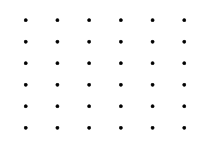
\includegraphics[width=\textwidth]{chp02_background/figures/gridpoints.pdf}
		\caption{An illustration of unresolved subgrid effects in a spatial discretisation.
			When a system is discretised, either from measurements or to numerically solve a model, processes between the grid points and no longer resolved or observed and yet can have a noticeable impact on the system.}
		\label{fig:subgrid_effects}
	\end{center}
\end{figure}


In particular, \citet{SuraEtAl_2005_MultiplicativeNoiseNonGaussianity} demonstrate that linear deterministic dynamics with multiplicative noise can be produce the non-Gaussian statistics that we observed in real systems.

The mathematical formulation of stochastic parameterisation -- where model predictions are now random quantities -- lends itself naturally to data assimilation \citep{BudhirajaEtAl_2019_AssimilatingDataModels,Jazwinski_2014_StochasticProcessesFiltering,LawEtAl_2015_DataAssimilationMathematical,ReichCotter_2015_ProbabilisticForecastingBayesian}, where ongoing observations are combined with predictions from a model to produce an improved forecast.
Data assimilation provides a framework that can simultaneously account for uncertainty in the observations and the model itself.
It has been shown that stochastic parameterisation can improve the quality of forecasts in data assimilation schemes \citep{MitchellGottwald_2012_DataAssimilationSlow,HaEtAl_2015_ComparisonModelError}.

\td{Flow from here into the need for maths - justifications, proofs, etc.?}
There is an emerging need to bridge the gap between mathematicians working on developing stochastic theory and algorithms, and the scientists looking to apply this work to their respective fields.
In particular, \citet{BernerEtAl_2017_StochasticParameterizationNew} conclude that ``geoscientists are often unaware of mathematically rigorous results that can aid in the development of physically relevant parameterizations, [while] mathematicians often do not know about open issues in scientific applications that might be mathematically tractable''.


Although stochastic parameterisation is more common in the atmospheric modelling context, oceanography also suffers from the same trade-off between spatial resolution and accuracy of predictions.

In the context of a fluid, unresolved processes can be vortices, eddies and turbulence \citep{Griffa_1996_ApplicationsStochasticParticle}.

The mixing effect that these eddies have on the surrounding flow can be modelled with spatiotemporally-varying diffusion \citehere, which via the Fokker-Planck equation can be equivalently formulated as a stochastic differential equation with multiplicative noise.
The Lagrangian trajectories, incorporating these unresolved eddy effects, are then modelled as solutions to the stochastic differential equation.
Equivalently, through the Fokker-Planck equation we can consider the evolution of a passive tracer undergoing advection due to the deterministic drift and diffusion from both any natural diffusivity and the unresolved processes.
The probability density function that solves the Fokker-Planck equation can be instead thought of as a time-varying density (with the appropriate normalisation) of the tracer.
For instance, the Fokker-Planck equation has been used to model the transport of ??? with a stochastic framework \citehere.
Hence, understanding the evolution of solutions to a stochastic differential equation is valuable in oceanography, as a means of quantifying both observational error and unresolved subgrid processes.


There are several different methods for quantifying eddy diffusivity given either observed tracer data or a global ocean circulation model.

The simplest notion of eddy diffusivity is a defined by






A recent approach by \cite{YingEtAl_2019_BayesianInferenceOcean} uses Bayesian inference to estimate the eddy diffusivity tensor from observed Lagrangian tracer data, by numerically solving the Fokker-Planck equation to compute a likelihood function.


In summary, stochastic parameterisation



\section{Limitations of stochastic simulation}
The introduction of stochastic terms complicates both the analytical treatment of the model.
For example, we saw in \Cref{sec:sde_theory} that adding even additive and  stationary\lb{Is this the right word?? I mean that \(\sigma\) is constant, with no time-dependency}\td{need to define additive versus multiplicative properly.} noise to an analytically solvable non-linear deterministic model can make exact solutions intractable.
Thus, across many applications the state of the art approach is to generate samples of the stochastic model and perform statistical inference.
For example, Monte-Carlo simulation is used across weather forecasting \citep{LeutbecherEtAl_2017_StochasticRepresentationsModel}, \td{something atmospheric} and \td{something oceanic}.

However, the most significant drawback of bulk stochastic simulation is the computational load.
In general, a large number of samples is required for convergent statistics and accurate inference, as discussed by \citet{Leutbecher_2019_EnsembleSizeHow}.
For a complex model, the computational load of computing a single realisation

The recent review by \citet{LeutbecherEtAl_2017_StochasticRepresentationsModel} highlights the need to develop computationally efficient schemes for quantifying stochasticity in weather and climate forecast models.


\td{Show the plateauing out that I am observing empirically when using a KDE . . . some literature on this?? This is a huge point to make}
For example, suppose that we intend on using the probabilistic forecast of our stochastic model in an inference scheme, such as in data assimilation in which model predictions are combined with ongoing observations to produce an improved forecast \cite[e.g.]{LawEtAl_2015_DataAssimilationMathematical,BudhirajaEtAl_2019_AssimilatingDataModels, ReichCotter_2015_ProbabilisticForecastingBayesian}.
This requires a probability density function or similar for our forecast, but in generating samples we initially only have a collection of finite discrete points.


The overall aim of this thesis is to address this problem, by developing characterisations of uncertainty and algorithms for approximating solution probability densities (as opposed to just generating samples) that are computationally efficient.
We aim to take advantage of the computational ease of generating solutions to a deterministic system (relative to taking many samples of a stochastic one).


The purpose of this example was to highlight the importance of accounting for measurement error and unresolved processes in a ; when the dynamics are complicated, then any uncertainty can have a significant impact on our inferences from the model, both quantitatively and qualitatively.



\section{Stochastic sensitivity}


\subsection{Current applications \& shortcomings}
Since stochastic sensitivity is only a recent development, it has only been applied in a limited number of places so far.
Here, we briefly review the literature in which the original formulation stochastic sensitivity by \citet{Balasuriya_2020_StochasticSensitivityComputable} has been applied.

\begin{itemize}
	\item \citet{Balasuriya_2020_UncertaintyFinitetimeLyapunov} uses stochastic sensitivity to compute an error bound for the finite-time Lyapunov (FTLE) computation.
	      The computable \(S^2\) value is used as an estimate of the standard deviation of the deviation between the deterministic and ``true'' (stochastic) trajectories, leading to a computable error bound on the FTLE value.


	\item \citet{FangEtAl_2020_DisentanglingResolutionPrecision}


	\item \citet{BadzaEtAl_2023_HowSensitiveAre} investigate the impact of velocity uncertainty on Lagrangian coherent structures (e.g. see the reviews by \citet{BalasuriyaEtAl_2018_GeneralizedLagrangianCoherent} and \citet{HadjighasemEtAl_2017_CriticalComparisonLagrangian}) extracted as robust sets with stochastic sensitivity.
	      The stochastic model \eqref{eqn:ss_sde} is used to generate realisations of Lagrangian trajectories subject to noise on the velocity field.
	      By directly capturing such uncertainty as a means of coherent set \citet{BadzaEtAl_2023_HowSensitiveAre} showed that robust sets extracted with stochastic sensitivity do SOMETHING.

\end{itemize}
There are several limitations to the work as originally presented by \citet{Balasuriya_2020_StochasticSensitivityComputable},
\begin{enumerate}
	\item The tools are restricted to two-dimensional models, and the constructions using projections have no obvious extension to \(n\)-dimensions.
	      Extending stochastic sensitivity to \(n\)-dimensions will enable application to a much broader class of models beyond the fluid flow context, including high-dimensional climate models.

	\item \citet{Balasuriya_2020_StochasticSensitivityComputable} only computes the expectation and variance of the projections \(P_\epsilon(x,\theta)\), which does not give us the distribution under the limit as \(\epsilon\) approaches 0.

	\item The computational formula for the anisotropic uncertainty and stochastic sensitivity, as described in \Cref{thm:orig_s2_calculation}, require knowledge of the divergence \(\nabla\cdot u\) of the velocity field, and computation of four integrals.
\end{enumerate}
